\documentclass[tikz,border=10pt]{standalone}
\usepackage[utf8]{inputenc}
\usepackage[T1]{fontenc}
\usepackage{lmodern}
\usetikzlibrary{arrows.meta,positioning,fit,calc}
\definecolor{navy}{HTML}{15324B}
\definecolor{blue}{HTML}{2F80C1}
\definecolor{cyan}{HTML}{DCEFF7}
\definecolor{orange}{HTML}{E8873A}
\definecolor{green}{HTML}{3B8F72}
\definecolor{red}{HTML}{B84A4A}
\tikzset{
  box/.style={draw=navy,rounded corners=3pt,very thick,align=center,
    minimum width=2.85cm,minimum height=1.15cm,text width=2.55cm,
    fill=white,font=\sffamily\small},
  arr/.style={-{Latex[length=2.5mm]},very thick,navy},
  note/.style={font=\sffamily\footnotesize,align=center,text=navy},
  title/.style={font=\sffamily\bfseries,align=center,text=navy}
}
\begin{document}
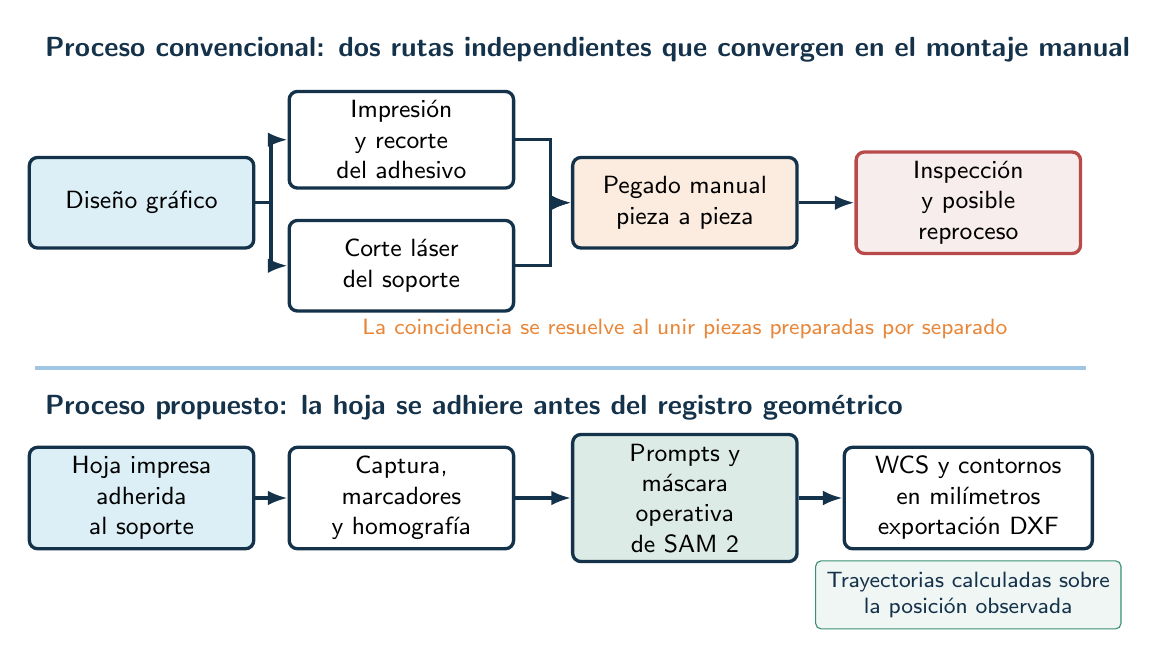
\begin{tikzpicture}[x=1cm,y=1cm]
  \node[title,anchor=west] at (-0.45,4.65)
    {Proceso convencional: dos rutas independientes que convergen en el montaje manual};
  \node[box,fill=cyan] (design) at (0.9,2.7) {Diseño gráfico};
  \node[box] (print) at (4.2,3.5) {Impresión y recorte\\del adhesivo};
  \node[box] (base) at (4.2,1.9) {Corte láser\\del soporte};
  \node[box,fill=orange!16] (assembly) at (7.8,2.7) {Pegado manual\\pieza a pieza};
  \node[box,fill=red!10,draw=red] (inspect) at (11.4,2.7)
    {Inspección y posible\\reproceso};
  \draw[arr] (design.east) -- ++(0.2,0) |- (print.west);
  \draw[arr] (design.east) -- ++(0.2,0) |- (base.west);
  \draw[arr] (print.east) -- ++(0.45,0) |- (assembly.west);
  \draw[arr] (base.east) -- ++(0.45,0) |- (assembly.west);
  \draw[arr] (assembly)--(inspect);
  \node[note,text=orange] at (7.8,1.1)
    {La coincidencia se resuelve al unir piezas preparadas por separado};

  \draw[blue!45,very thick] (-0.45,0.6)--(12.9,0.6);
  \node[title,anchor=west] at (-0.45,0.1)
    {Proceso propuesto: la hoja se adhiere antes del registro geométrico};
  \node[box,fill=cyan] (laminate) at (0.9,-1.05)
    {Hoja impresa\\adherida al soporte};
  \node[box] (capture) at (4.2,-1.05)
    {Captura, marcadores\\y homografía};
  \node[box,fill=green!18] (sam) at (7.8,-1.05)
    {Prompts y máscara\\operativa de SAM 2};
  \node[box,minimum width=3.15cm,text width=2.85cm] (geometry) at (11.4,-1.05)
    {WCS y contornos\\en milímetros\\exportación DXF};
  \draw[arr] (laminate)--(capture);
  \draw[arr] (capture)--(sam);
  \draw[arr] (sam)--(geometry);
  \node[note,draw=green,rounded corners=2pt,fill=green!8,inner sep=4pt]
    at (11.4,-2.28)
    {Trayectorias calculadas sobre\\la posición observada};
\end{tikzpicture}
\end{document}
